\newpage
\section{Problem 2: IMAGE ENHANCEMENT}\label{problem-2-image-enhancement}
Original image \cref{fig2} for question \textbf{(a)}, \textbf{(b)} \& \textbf{(c)}.
\begin{figure}
    \centering
    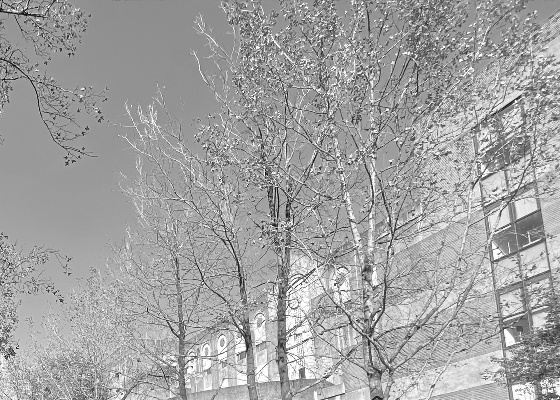
\includegraphics[width=0.7\textwidth]{image/sample2.jpg}
    \caption{\textbf{sample2.jpg}}
    \label{fig2}
\end{figure}

% a
\textbf{(a)} Decrease the brightness of \textbf{sample2.jpg} by {dividing the
intensity values by 5} and output the image as \textbf{3\_result.jpg}.

\textbf{Motivation}
Looks how to dim the image.

\textbf{Approach}
\begin{enumerate}
  \item Load image as \texttt{numpy\ array/matrix}.
  \item Divide intensity values, i.e.~values in matrix by $5$.
  \item Save image as \textbf{3\_result.jpg}.
\end{enumerate}

\textbf{Performance of results}
Result of problem 2(a): \textbf{3\_result.jpg} \cref{fig2a}.
\begin{figure}
    \centering
    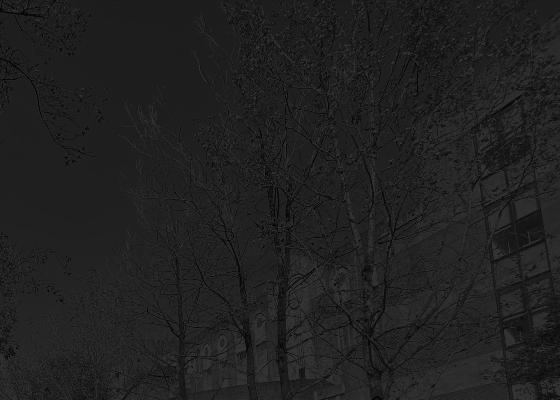
\includegraphics[width=0.7\textwidth]{image/3_result.jpg}
    \caption{\textbf{3\_result.jpg} Intensity $\times 5$}
    \label{fig2a}
\end{figure}

\textbf{Discussion}
It looks dark.

% b
\textbf{(b)} Increase the brightness of \textbf{3\_result.jpg} by multiplying the intensity values by 5 and output the image as \textbf{4\_result.jpg}.

\textbf{Motivation}
Looks how to turn the image brighter.

\textbf{Approach}
It is similar to problem \textbf{(a)}. Actually we give \(5\) times from \textbf{3\_result.jpg} s.t. The dynamic range of \textbf{4\_result.jpg} is similar to \textbf{sample2.jpg}.

\textbf{Performance of results}
Result of problem 2(b): \textbf{4\_result.jpg} \cref{fig2b}.
\begin{figure}
    \centering
    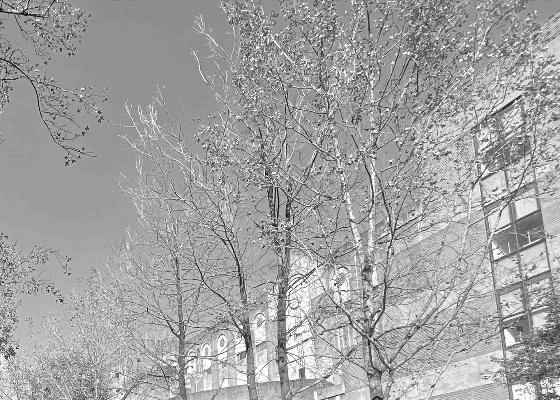
\includegraphics[width=0.7\textwidth]{image/4_result.jpg}
    \caption{\textbf{4\_result.jpg} Intensity $\div 5$}
    \label{fig2b}
\end{figure}

\textbf{Discussion}
It looks as the same as original image. (Really!?)

% c
\textbf{(c)} {Plot the histograms} of \textbf{sample2.jpg}, \textbf{3\_result.jpg} and \textbf{4\_result.jpg}. What can you observe from these three
histograms?

\textbf{Motivation}
Compare with \cref{fig2,fig2a,fig2b}. Is there any change after we conduct $\times / \div 5$?

\textbf{Approach}
My approach is
\begin{enumerate}
  \item Define \texttt{intensity\_hist} that returns \textbf{intensity} with \textbf{counts} of the image.
\end{enumerate}
Note: We need to be careful of converting \textbf{float} and \textbf{int}. I use \texttt{numpy.uint8} here.

\textbf{Performance of results}
Result of problem 2(c): \cref{fig2c}.
\begin{figure}
  \centering
  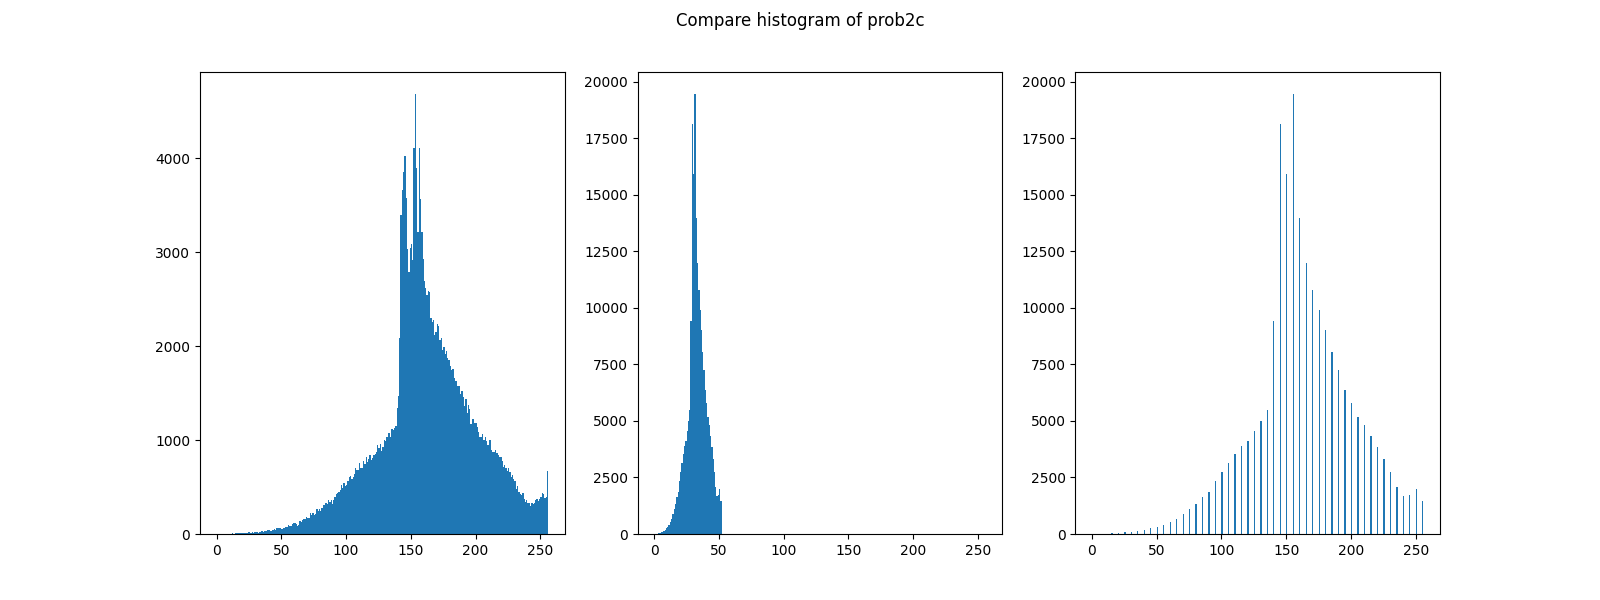
\includegraphics[width=\textwidth]{image/prob2c.png}
  \caption{Histogram of \textbf{sample2.jpg} family}
  \label{fig2c}
\end{figure}

\textbf{Discussion}
According to \cref{fig2c}, we can find out
\begin{enumerate}
\def\labelenumi{\arabic{enumi}.}
\tightlist
\item \textbf{3\_result.jpg} (center histogram) is obviously dark than \textbf{sample2.jpg} (left histogram). And its dynamic range (range of intensity) is smaller.
\item \textbf{sample2.jpg} and \textbf{4\_result.jpg} are similar but \textbf{4\_result.jpg} (right histogram) is \alert{sparse}. As we multiple \(5\) from \textbf{3\_result.jpg} which compress the dynamic range and loss some intensity when converting to \texttt{np.uint8}.
\end{enumerate}

% --------------------------------------------------------------------
\rule{\textwidth}{.5mm}
Original image \cref{fig2_1} for question \textbf{(d)}, \textbf{(e)} \& \textbf{(f)}.
\begin{figure}
    \centering
    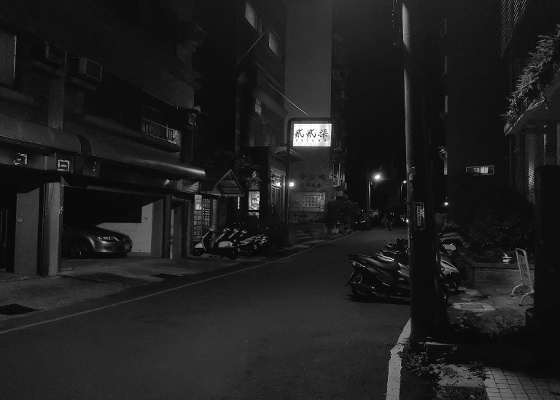
\includegraphics[width=0.7\textwidth]{image/sample3.jpg}
    \caption{\textbf{sample3.jpg}}
    \label{fig2_1}
\end{figure}

% d
\textbf{(d)} Perform global histogram equalization (GHE) on \textbf{sample3.jpg} and
output the results as \textbf{5\_result.jpg}.

\textbf{Motivation}
It seems that original is too \textbf{dark} and some detail in the region is vague. Let us increase \textbf{contrast} of intensity.

\textbf{Approach}
Based on \textbf{Transfer function} in \textit{Lec 2 page 16}.
My approach is
\begin{enumerate}
\def\labelenumi{\arabic{enumi}.}
\tightlist
\item Count probability distribution function (pdf) of intensity and accumulate as cumulative distribution function (cdf).
\item Define \textbf{transfer function} as \\
\texttt{s\ =\ np.array(\ np.round(\ (L\ -\ 1)\ *\ cdf),\ dtype=np.uint8\ );\ res=s{[}r{]}} \\
It finds the equal value of cdf between input intensity and desired uniform distribution. Then get look-up table.
\item Do transfer function on whole image.
\end{enumerate}

\textbf{Performance of results}
Result of problem 2(d): \textbf{5\_result.jpg} \cref{fig2d}.
\begin{figure}
    \centering
    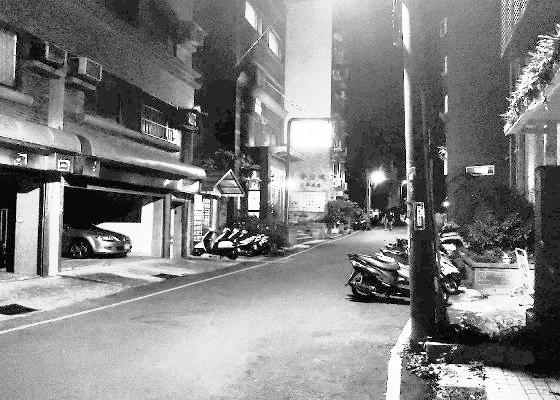
\includegraphics[width=0.7\textwidth]{image/5_result.jpg}
    \caption{\textbf{5\_result.jpg} GHE}
    \label{fig2d}
\end{figure}

\textbf{Discussion}
We could see \cref{fig2d} after increase its contrast:
\begin{enumerate}
  \item The \textit{car}, \textit{motorcycle} and \textit{buildings} are obvious.
  \item The kanban ``貳貳柒'' is too bright to look.
  \item The kanban which is bellow ``貳貳柒'' is more clear.
\end{enumerate}

% e
\textbf{(e)} Perform local histogram equalization (LHE) on \textbf{sample3.jpg} and output the results as \textbf{6\_result.jpg}.

\textbf{Motivation}
According to the \href{https://www.imageeprocessing.com/2011/06/local-histogram-equalization.html}{MATLAB reference}.
The idea is to conduct histogram equalization on \textbf{local masking array}.

\textbf{Approach}
My approach is 
\begin{enumerate}
  \item Expand the \textbf{image array} accroding to \emph{kernel\_size}~\(k=51\). In practice, expand boundary with \(25= \lfloor \frac{51}{2} \rfloor\).
  \item Collect the \textbf{sub arrays} from \textbf{expanded image array}.
  \item Conduct the \textbf{histogram equalization} on each \textbf{sub array}.
\end{enumerate}

\textbf{Performance of results}
Result of problem 2(e): \textbf{6\_result.jpg} \cref{fig2e}.
\begin{figure}
    \centering
    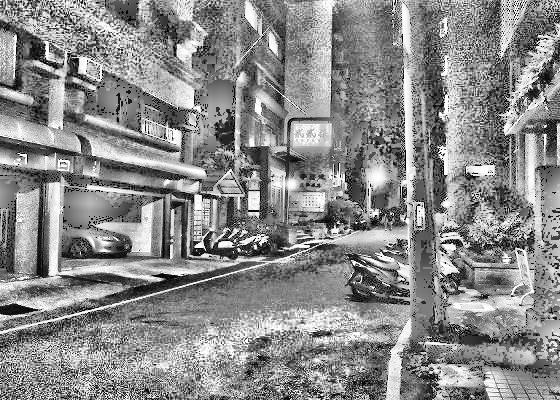
\includegraphics[width=0.7\textwidth]{image/6_result.jpg}
    \caption{\textbf{6\_result.jpg} LHE with $k=51$}
    \label{fig2e}
\end{figure}

\textbf{Discussion}
We could see \cref{fig2e} that
\begin{enumerate}
  \item Two kanbans are visible.
  \item But there are a lot of \textbf{furry} regions that are not clear than before. Especially in large region, such as \textit{road}, \textit{buildings} and \textit{sky}.
\end{enumerate}

Futhermore, we could discuss the results of different \textit{kernel size}~\(k\).
From $k=3$
\begin{figure}
  \centering
  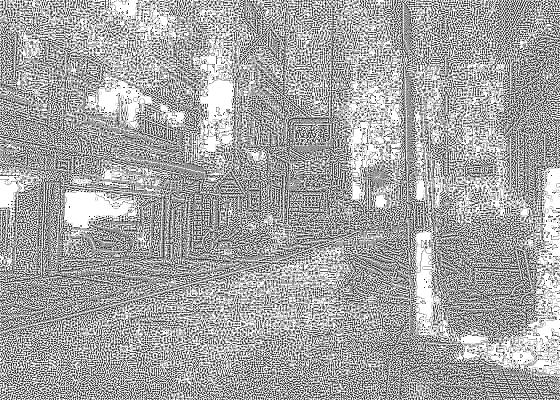
\includegraphics[width=0.7\textwidth]{image/tmp/6_result_0.jpg}
  \caption{LHE with kernel size $3$}
  \label{fig2e_1}
\end{figure}
, $k=5$
\begin{figure}
  \centering
  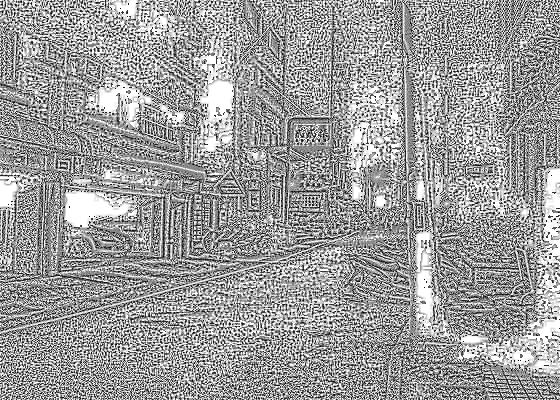
\includegraphics[width=0.7\textwidth]{image/tmp/6_result_1.jpg}
  \caption{LHE with kernel size $5$}
  \label{fig2e_2}
\end{figure}
, $k=151$
\begin{figure}
  \centering
  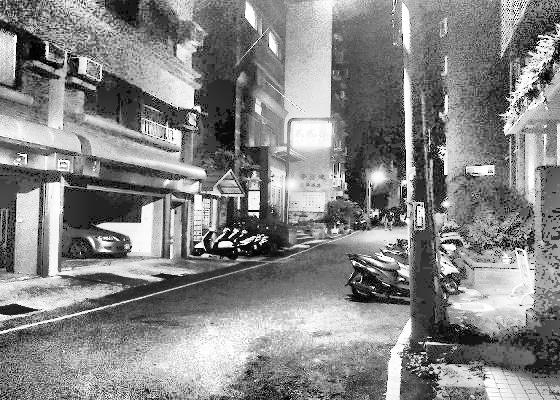
\includegraphics[width=0.7\textwidth]{image/tmp/6_result_3.jpg}
  \caption{LHE with kernel size $151$}
  \label{fig2e_3}
\end{figure}
\& $k=351$.
\begin{figure}
  \centering
  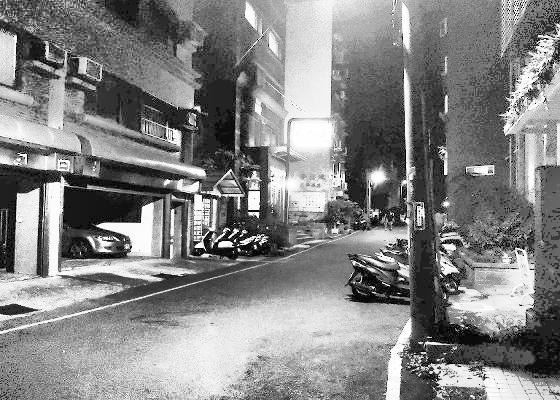
\includegraphics[width=0.7\textwidth]{image/tmp/6_result_4.jpg}
  \caption{LHE with kernel size $351$}
  \label{fig2e_4}
\end{figure}
We could see smaller $k$ give us images like \textbf{sand painting}; The larger $k$ give us more clear but the kanban ``貳貳柒'' becomes brighter.

And here is their histograms \cref{fig2e_hist}:
\begin{figure}
  \centering
  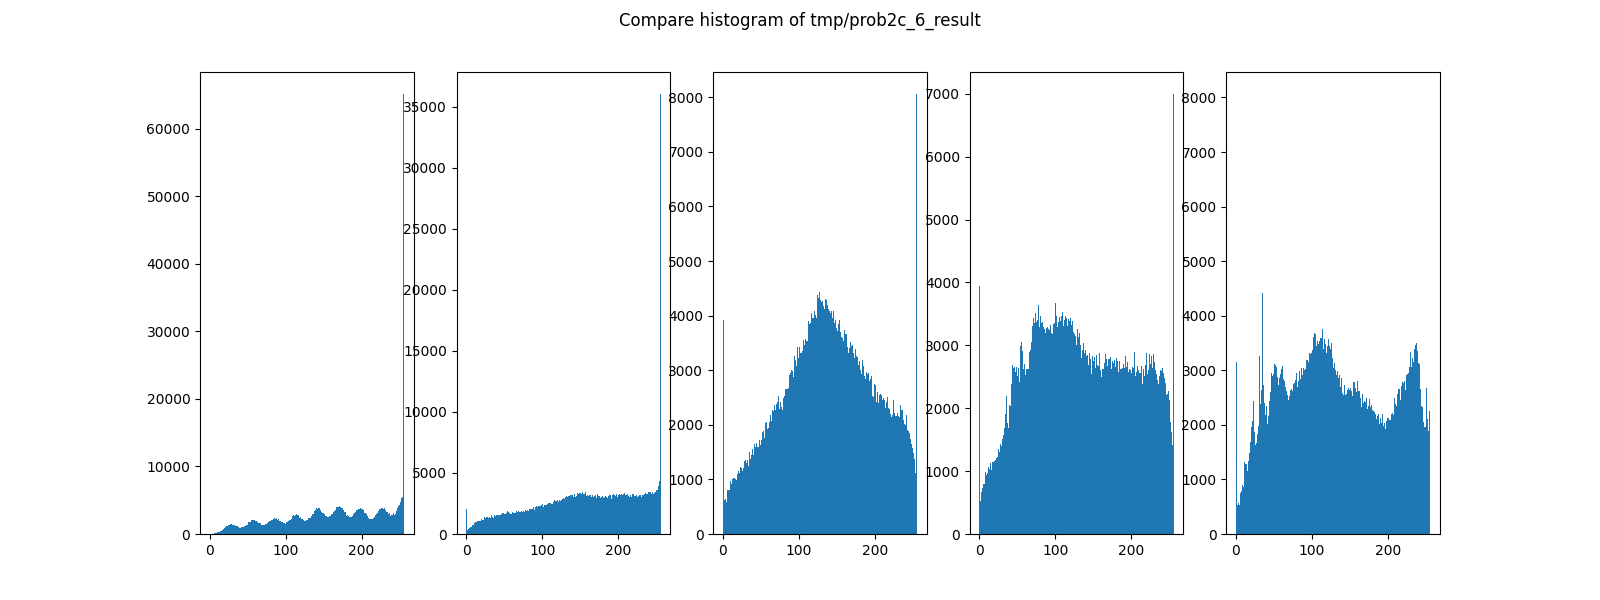
\includegraphics[width=0.7\textwidth]{image/tmp/prob2c_6_result.png}
  \caption{Histograms of different kernel size ($k=3,5,51,151,351$)}
  \label{fig2e_hist}
\end{figure}
It shows that after we increase $k$, the dynamic range would \textbf{shift to left} and uniform.
In the end, I feel that $k=51$ is good as its central shape.

% f
\textbf{(f)} Plot the histograms of \textbf{5\_result.jpg} and \textbf{6\_result.jpg}. What is the main difference between local and global histogram equalization?

\textbf{Motivation}
Compare with \cref{fig2_1,fig2d,fig2e}. What is difference between global and local histogram equalization.

\textbf{Approach}
It is the same as \textbf{2(c)}.

\textbf{Performance of results}
Result of problem 2(f): \cref{fig2f}.
\begin{figure}
  \centering
  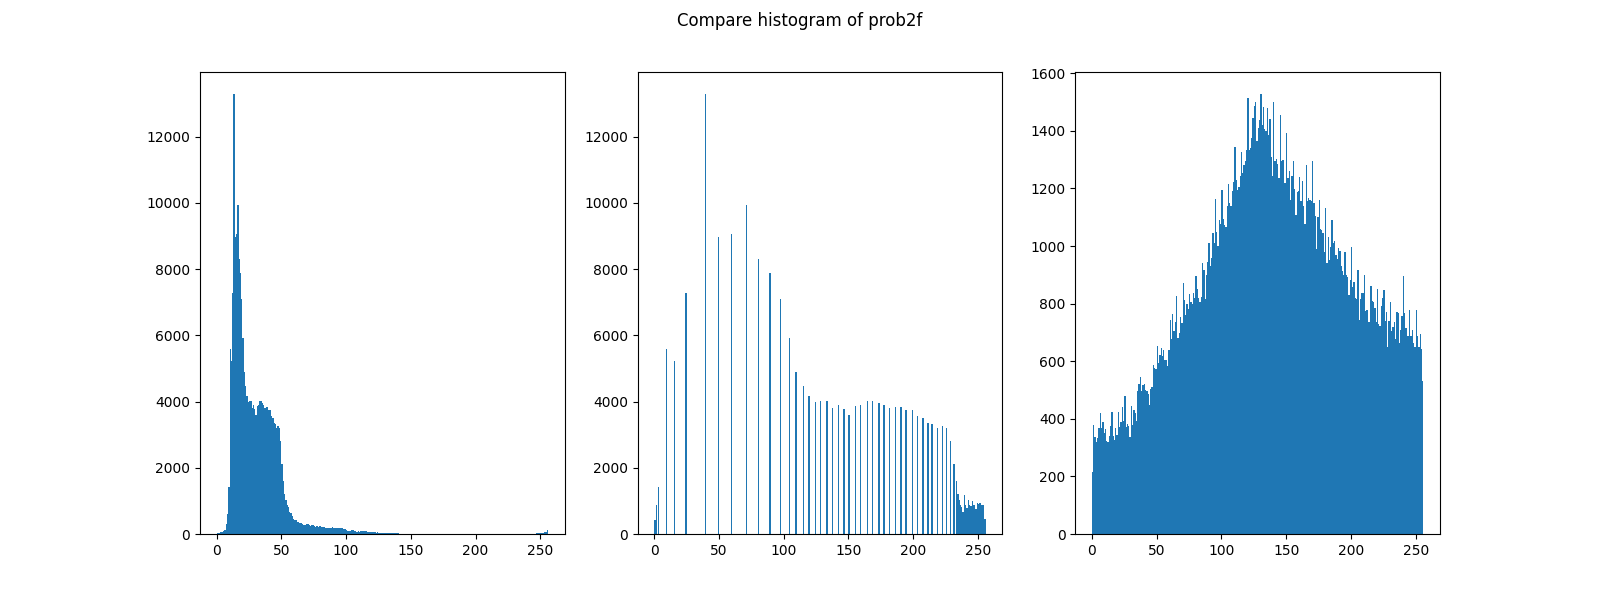
\includegraphics[width=\textwidth]{image/prob2f.png}
  \caption{\textbf{sample3.jpg} family}
  \label{fig2f}
\end{figure}

\textbf{Discussion}
According to \cref{fig2f}, we could see the \alert{difference} between \textbf{5\_result.jpg} and \textbf{6\_result.jpg}:
\begin{itemize}
\tightlist
\item \textbf{5\_result.jpg}(center) is more \alert{sparse} than \textbf{6\_result.jpg}(right).
\item The dense region of \textbf{5\_result.jpg}(center) is larger than \textbf{6\_result.jpg}(right).
\item The distribution of intensity in \textbf{6\_result.jpg}(right) is \alert{concentrate}.
\item In summary of \textbf{6\_result.jpg}, I consider that we make some region more contrast. Such as kanban of ``貳貳柒''. But for larger region, it seems more vague than original graph.
\end{itemize}

% --------------------------------------------------------------------
\rule{\textwidth}{.5mm}
Original image \cref{fig2_2} for question \textbf{(g)}.
\begin{figure}
    \centering
    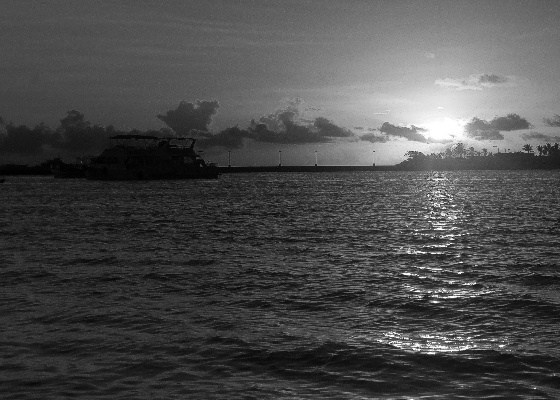
\includegraphics[width=0.7\textwidth]{image/sample4.jpg}
    \caption{\textbf{sample4.jpg}}
    \label{fig2_2}
\end{figure}

\textbf{(g)} Please design a transfer function to enhance \textbf{sample4.jpg} as best as you can. Output the result as \textbf{7\_result.jpg} and specify all the parameters.

\textbf{Motivation}
I want to make the \textit{ship} more visible. But keep the \textit{sunrise} clearly i.e. not too bright.

\textbf{Approach}
My last choice is \textbf{Rubber Band with power transfer}.
The transfer function with parameters is defined as
\begin{equation}
  G(j, k) = 
  \begin{cases}
    \left[F(j, k) \right]^{ \frac{1}{2} },& \text{if } 0 \leq F(j, k) \leq 0.7 \\
    0.83 + \left[F(j, k) \right]^{2},& \text{if } 0.7 \leq F(j, k) \leq 1
  \end{cases}
\end{equation}
Note: \((0.7, 0.83)\) is \textbf{inflection point/control point}.

And \cref{fig2g_T} is how my transfer function looks like:
\begin{figure}
\centering
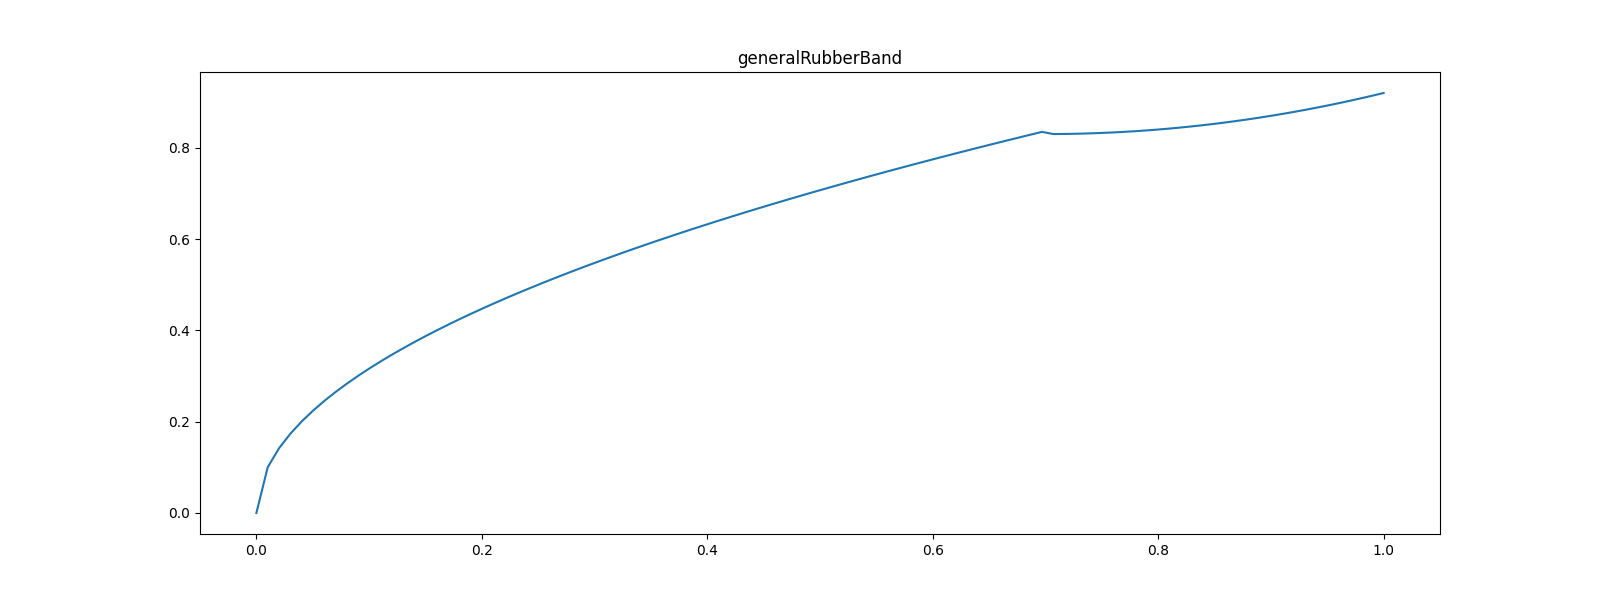
\includegraphics[width=\textwidth]{image/prob2g_transfer_generalRubberBand.png}
\caption{image alt}
\label{fig2g_T}
\end{figure}

\textbf{Performance of results}
Result of problem 2(g): \textbf{7\_result.jpg} \cref{fig2g}.
\begin{figure}
    \centering
    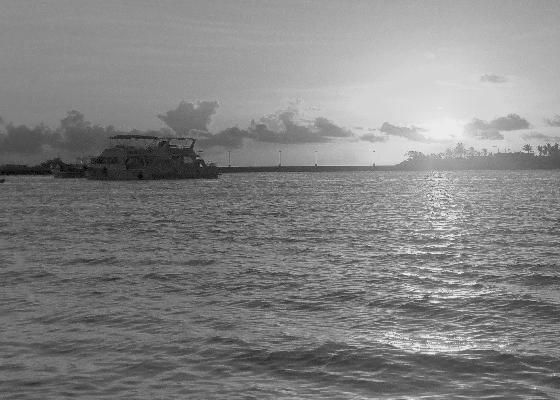
\includegraphics[width=0.7\textwidth]{image/7_result.jpg}
    \caption{\textbf{7\_result.jpg} Rubber band with power transfer}
    \label{fig2g}
\end{figure}

\textbf{Discussion}
We start from \cref{fig2g_hist}, it shows the before-after histograms.
\begin{figure}
\centering
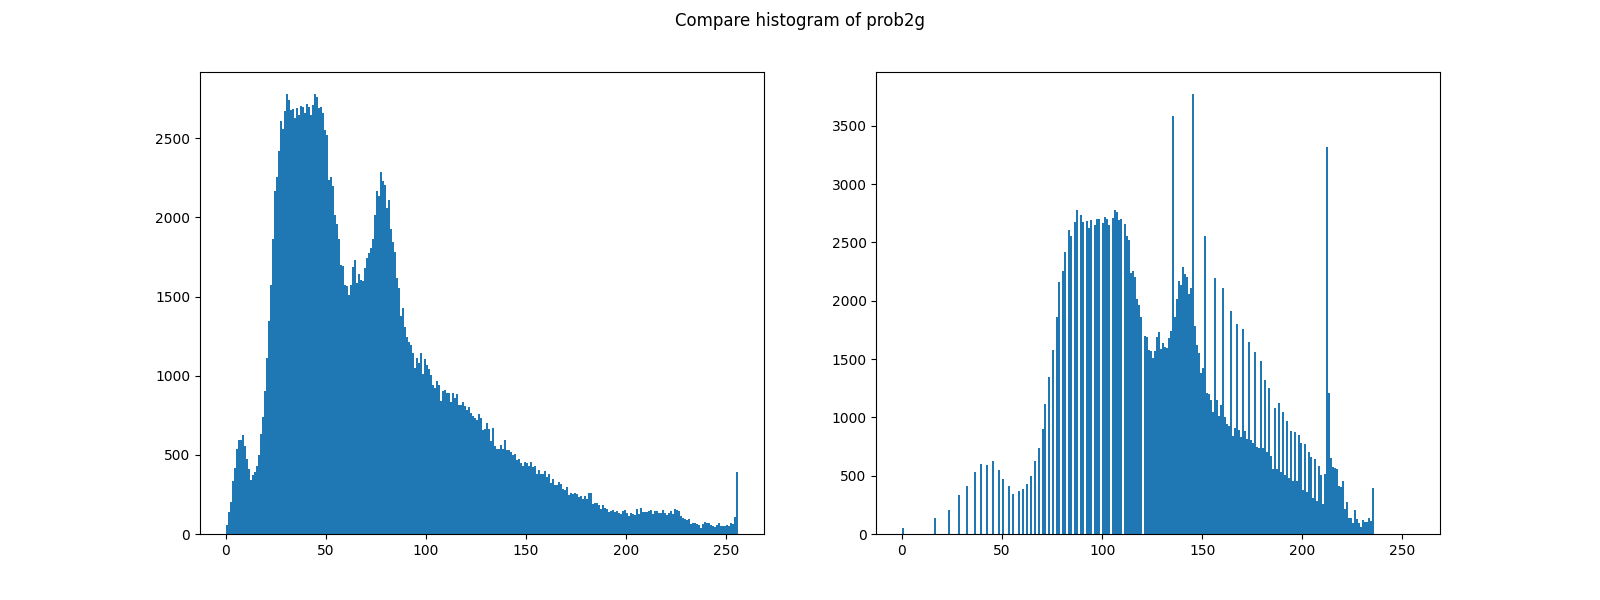
\includegraphics[width=\textwidth]{image/prob2g.png}
\caption{\textbf{sample4.jpg} family}
\label{fig2g_hist}
\end{figure}
I conclude that
\begin{itemize}
\tightlist
\item As I consider the original graph is \textbf{too dark} at region of \textit{ship} and \textbf{left side} of \textit{ocean}.
\item But I want to keep the \textbf{bright} region of \textit{sunrise} clearly.
\item After I try some transfer functions, I feel rubber band with power transfer is good! As I could design the \textbf{control point} to decide the change/slope of bright and dark intensity region.
\end{itemize}

\textbf{More transfer functions}

I list some transfer functions in \textit{Lec 2}.

\textbf{Power Law} \cref{fig2g_t1}.
\begin{figure}
  \centering
  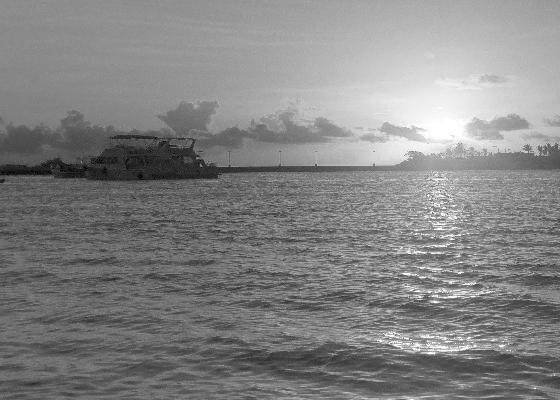
\includegraphics[width=0.5\textwidth]{image/tmp/7_result_1.jpg}
  \caption{Power Law with $p=\frac{1}{2}$}
  \label{fig2g_t1}
\end{figure}

\textbf{Rubber band (linear)} \cref{fig2g_t2}.
\begin{figure}
  \centering
  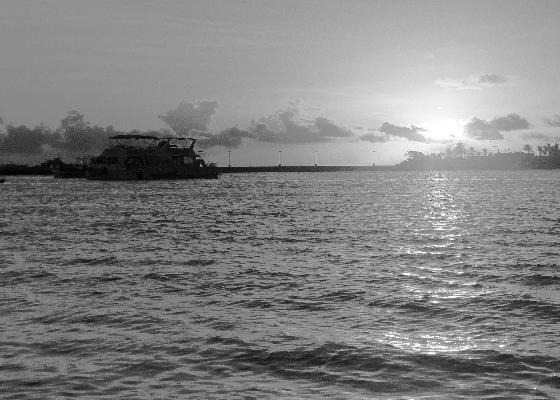
\includegraphics[width=0.5\textwidth]{image/tmp/7_result_2.jpg}
  \caption{Rubber band with critical point $(0.2, 0.5)$}
  \label{fig2g_t2}
\end{figure}

\textbf{Log Pt} \cref{fig2g_t3}.
\begin{figure}
  \centering
  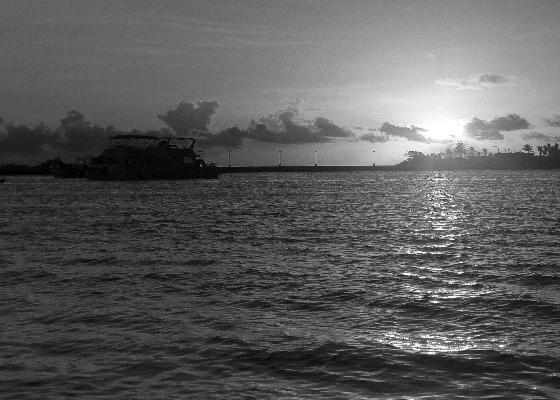
\includegraphics[width=0.5\textwidth]{image/tmp/7_result_3.jpg}
  \caption{logPt with $a=1$}
  \label{fig2g_t3}
\end{figure}

\textbf{Log Pt} \cref{fig2g_t6}.
\begin{figure}
  \centering
  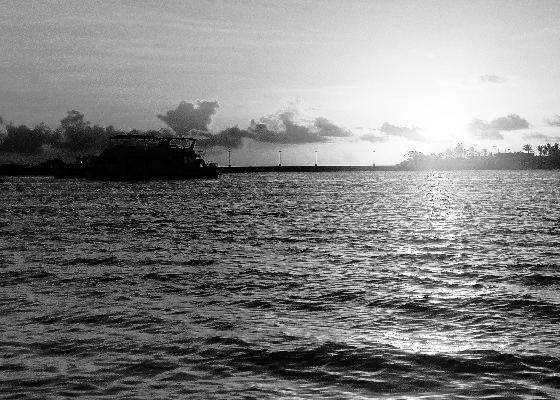
\includegraphics[width=0.5\textwidth]{image/tmp/7_result_6.jpg}
  \caption{Global histogram equalization}
  \label{fig2g_t6}
\end{figure}
